\documentclass[../main.tex]{subfiles}
\begin{document}

\chapter{MATLAB Basics}
\addcontentsline{toc}{section}{Chapter 1: MATLAB Basic}

\section{ WHAT IS MATLAB?}

\noindent As a student who has already taken courses at least up through calculus, you most
likely have seen the power of graphing calculators and perhaps those with
symbolic capabilities. MATLAB adds a whole new exciting set of capabilities as
a powerful computing tool. Here are a few of the advantages you will enjoy when
using MATLAB, as compared to a graphing calculator:

\begin{enumerate}
\item It is easy to learn and use. You will be entering commands on your big,
familiar computer keyboard rather than on a tiny little keypad where
sometimes each key has four different symbols attached.
\item The graphics that MATLAB produces are of very high resolution. They can
be easily copied to other documents (with simple clicks of your mouse) and
printed out in black/white or color format. The same is true of any numerical
and algebraic MATLAB inputs and outputs.
\item MATLAB is an abbreviation for MATrix LABoratory. It is ideally suited for
calculations and manipulations involving matrices. This is particularly useful
for computer users since the spreadsheet (the basic element for recording data
on a computer) is just a matrix.
\item MATLAB has many built-in programs and you can interactively use them to
create new programs to perform your desired tasks. It enables you to take
advantage of the full computing power of your computer, which has much
more memory and speed than a graphing calculator.
\item MATLAB's language is based on the C-family of computer languages.
People experienced with such languages will find the transition to MATLAB
natural and people who learn MATLAB without much computer background
will, as a fringe benefit, be learning skills that will be useful in the future if
they need to learn more computer languages.
\item MATLAB is heavily used by mathematicians, scientists, and engineers and
there is a tremendous amount of interesting programs and information
available on the Internet (much of it is free). It is a powerful computing
environment that continues to evolve.
\end{enumerate}

We wish here and now to present a disclaimer. MATLAB is a spectacularly vast
computing environment and our plan is not to discuss all of its capabilities, but
rather to give a decent survey of enough of them so as to provide the reader with a
powerful new arsenal of uses of MATLAB for solving a variety of problems in
mathematics and other sciences. Several good books have been written just on
using MATLAB; see, for example, references [HiHi-00], [HuL¡Ro-01], [PSMI98], and[HaLi-00].\footnote[1]{Citations in square brackets refer to items in the References section in the back of this book} 

\section{STARTING AND ENDING A MATLAB SESSION}

We assume that MATLAB has been installed on the system that you are using.\footnote[2]{MATLAB is available on numerous computing platforms including PC Windows, Linux, MAC,
Solaris, Unix, HP-UX. The functionality and use is essentially platform independent although some
external interface tasks may vary.}
Instructions for starting MATLAB are similar to those for starting any installed
software on your system. For example, on most windows-based systems, you
should be able to simply double click on MATLAB's icon. Once MATLAB is
started, a command window should pop up with a \textbf {prompt:}» (or EDU » if you
are using the Student Version). In what follows, if we tell you to enter something
like » 2+2 (on the command window), you enter 2+2 only at the prompt—
which is already there waiting for you to type something. Before we begin our
first brief tutorial, we point out that there is a way to create a file containing all
interactions with a particular MATLAB session. The command diar y will do
this. Here is how it works: Say you want to save the session we are about to start
to your floppy disk, which you have inserted in the a:/-drive. After the prompt
type: 

\begin{verbatim}
>> diary a:/tutorl.txt
\end{verbatim}

\noindent NOTE: If you are running MATLAB in a computer laboratory or on someone
else's machine, you should always save things to your portable storage device or
personal account. This will be considerate to the limitations of hard drive space on
the machines you are using and will give you better assurance that the files still
will be available when you need them. 


This causes MATLAB to create a text file called tutorl . tx t in your a:/- drive
called tutorl . txt , which, until you end the current MATLAB session, will be
a carbon copy of your entire session on the command window. You can later
open it up to edit, print, copy, etc. It is perhaps a good idea to try this out once to
see how it works and how you like it (and we will do this in the next section), but
in practice, most MATLAB users will often just copy the important parts, of their
MATLAB session and paste them appropriately in an open word processing
window of their choice.


On most platforms, you can end a MATLAB session by clicking down your left
mouse button after you have moved the cursor to the "File" menu (located on the
upper-left comer of the MATLAB command window). This will cause a menu of
commands to appear that you can choose from. With the mouse button still held
down, slide the cursor down to the "Exit MATLAB" option and release it. This will end the session. Another way to accomplish the same would be to simply
click (and release) the left mouse button after you have slid it on top of the "X"
button at the upper-right corner of the command window. Yet another way is to
simply enter the command: 

\begin{verbatim}
>> quit 
\end{verbatim}

\noindent Any diary file you created in the session will now be accessible.

\section{A FIRST MATLAB TUTORIAL}

\noindent As with all tutorials we present, this is intended to be worked by the reader on a
computer with MATLAB installed. Begin by starting a MATLAB session as
described earlier. If you like, you may begin a diary as shown in the previous
section on which to document this session. MATLAB will not respond to or
execute any command until you press the "enter key," and you can edit a
command (say, if you made a typo) and press enter no matter where the cursor is
located in a given command line. Let us start with some basic calculations: First
enter the command:

\begin{verbatim}
>> 5 + 3
 -> ans = 8
\end{verbatim}

\noindent The arrow (->) notation indicates that MATLAB has responded by giving us
ans = 8. As a general rule we will print MATLAB input in a different font
(Courie r New) than the main font of the text (Times New Roman). It does not
matter to MATLAB whether you leave spaces around the + sign.\footnote[3]{ The format of actual output that MATLAB gives can vary slightly depending on the platform and
version being used. In general it will take up more lines and have more blank spaces than as we have
printed it. We adopt this convention throughout the book in order to save space.}
 (This is usually
just done to make the printout more legible.) Instead of adding, if we wanted to
divide 5 by 3, we would enter (the operation -5- is represented by the keyboard
symbol / in MATLAB)
 
 \begin{verbatim}
>> 5/3
-> ans =1.6667 
\end{verbatim}

The output "1.6667" is a four-decimal approximation to the unending decimal
approximation. The exact decimal answer here is 1.666666666666... (where the
6's go on forever). The four-decimal display mode is the default format in which
MATLAB displays decimal answers. The previous example demonstrates that if
the inputs and outputs are integers (no decimals), MATLAB will display them as
such. MATLAB does its calculations using about 16 digits—we shall discuss
this in greater detail in Chapters 2 and 5. There are several ways of changing how
your outputs are displayed. For example, if we enter: 

\begin{verbatim}
 >> format long 
>> 5/3
-> ans =1.66666666666667 
\end{verbatim}

\noindent we will see the previous answer displayed with 15 digits. All subsequent
calculations will be displayed in this format until you change it again. To change
back to the default format, enter » format short. Other popular formats are
» format bank (displays two decimal places, useful for applications to
finance) and » format rat (approximates all answers as fractions of small
integers and displays them as such). It is not such a good idea to work in
format ra t unless you know for sure the numbers you are working with are
fractions as opposed to irrational numbers, like 71 = 3.14159265..., whose
decimals go on forever without repetition and are impossible to express via
fractions.

In MATLAB, a single equals sign (=) stands for "is assigned the value." For
example, after switching back to the default format, let us store the following
constants into MATLAB's workspace memory: 

\begin{verbatim}
>>format short
>> a = 2.5
>> a = 2.5000 
>> b = 64
-> b = 64 
\end{verbatim}


Notice that after each of these commands, MATLAB will produce an output of
simply what you have inputted and assigned. You can always suppress the output
on any given MATLAB command by tacking on a semicolon (;) at the end of the
command (before you press enter). Also, you can put multiple MATLAB
commands on a single line by separating them with commas, but these are not
necessary after a semicolon. For example, we can introduce two new constants a a
and bb without having any output using the single line: 

\begin{verbatim}
>>aa = 11; bb = 4; 
\end{verbatim}

Once variables have been assigned in a MATLAB session, computations
involving them can be done using any of MATLAB's built-in functions. For
example, to evaluate aa + a$\sqrt{b}$ , we could enter

\begin{verbatim}
>> aa + a*sqrt(b)
>> ans=31
\end{verbatim}

\noindent Note that a a stands for the single variable that we introduced above rather than
a1, so the output should be 31. MATLAB has many built-in functions, many of
which are listed in the MATLAB Command Index at the end of this book. 

MATLAB treats all numerical objects as matrices, which are simply rectangular
arrays of numbers. Later we will see how easy and flexible MATLAB is in manipulating such arrays. Suppose we would like to store in MATLAB the
following two matrices:


\begin{equation*}
	A = 
	\begin{bmatrix}
	2 & 4 \\
	-1 & 6\\
	\end{bmatrix},
	 B =
	\begin{bmatrix}
	2 & 5 & -3 \\
	1 & 0 & -1 \\
	8 & 4 & -0 \\
	\end{bmatrix}
\end{equation*}

\noindent We do so using the following syntax:

\begin{verbatim}
>> A = [2 4 ; -1 6] 
->A= 
\end{verbatim}
\begin{tabular}{cc}
2&4\\
-1 &6 
\end{tabular} 

\begin{verbatim}

>> B = [2 5 -3 ; 1 0 -1 ; 8 4 0] 
>>-> B=
\end{verbatim}

\begin{tabular}{ccc}
2&5&-3\\
1&0&-1\\
8&4&0\\
\end{tabular} 

(note that the rows of a matrix are entered in order and separated by semicolons;
\noindent also, adjacent entries within a row are given at least one space between). You can
see from the outputs that MATLAB displays these matrices pretty much in their
mathematical form (but without the brackets). 

In MATLAB it is extremely simple to edit a previous command into a new one.
Let's say in the matrix B above, we wish to change the bottom-left entry from
eight to three. Since the creation of matrix B was the last command we entered,
we simply need to press the up-arrow key ($\uparrow$) once and magically the whole last
command appears at the cursor (do this!). If you continue to press this up-arrow
key, the preceding commands will continue to appear in order. Try this now!
Next press the down arrow key ($\downarrow$) several times to bring you back down again to
the most recent command you entered (i.e., where we defined the matrix B ). Now
simply use the mouse and/or left- and right-arrow keys to move the cursor to the 8
and change it to 3, then press enter. You have now overwritten your original
matrix for B with this modified version. Very nice indeed! But there is more. If
on the command line you type a sequence of characters and then press the uparrow key, MATLAB will then retrieve only those input lines (in order of most
recent occurrence) that begin with the sequence of characters typed. Thus for
example, if you type a and then up-arrow twice, you would get the line of input
where we set $aa = 11$.

A few more words about "variables" are in order. Variable names can use up to
19 characters, and must begin with a letter, but after this you can use digits and
underscores as well. For example, two valid variable names are
diffusion22tim e and Shock\_wave\_index; however, Final\$Amount
would not be an acceptable variable name because of the symbol \$. Any time that
you would like to check on the current status of your variables, just enter the
command who:

\begin{verbatim}
>> who 
->Your variables are:
 A B a aa ans b bb 
\end{verbatim}

\noindent For more detailed information about all of the variables in the workspace
(including the size of all of the matrices) use the command whos: 

\begin{verbatim}
 >> whos
\end{verbatim}
\noindent \begin{tabular}{cccc}
-»		name&size&bytes&class\\
		A&2x2&32 double&array\\

		B&3x3&72 double&array\\

		a&1x1&8 double&array\\

		aa&1x1&8 double&array\\

		ans&1x1&8 double&array\\

		b&1x1&8 double&array\\

		bb&1x1&8 double&array\\	
\end{tabular}

\vspace{0.25cm}

You will notice that MATLAB retains both the number a and the matrix A.
\underline{MATLAB is case-sensitive.} You will also notice that there is the variable ans in
the workspace. Whenever you perform an evaluation/calculation in MATLAB, an
automatic assignment of the variable ans is made to the most recent result (as the
output shows). To clear any variable, say aa, use the command

\begin{verbatim}
>> clear aa
\end{verbatim}

Do this and check with who that aa is no longer in the workspace. If you just
enter clear , all variables are erased from the workspace. More importantly,
suppose that you have worked hard on a MATLAB session and would like to
retain all of your workspace variables for a future session. To save (just) the
workspace variables, say to your floppy a:\ drive, make sure you have your disk
inserted and enter: 

\begin{verbatim}
>> save a:/tutvars 
\end{verbatim}

\noindent This will create a file on your floppy called tutvars.ma t (you could have
called it by any other name) with all of your variables. To see how well this
system works, go ahead and quit this MATLAB session and start a new one. If
you type who you will get no output since we have not yet created any variables in
this new session. Now (making sure that the floppy with tutvar s is still
inserted) enter the command: 

\begin{verbatim}
>> load a:/tutvars  
\end{verbatim}

\noindent If you enter who once again you will notice that all of those old variables are now
in our new workspace. You have just made it through your first MATLAB
tutorial. End the session now and examine the diary file if you have created one. \\

If you want more detailed information about any particular MATLAB command,
say who, you would simply enter: 

\begin{verbatim}
>>help who 
\end{verbatim}

\noindent and MATLAB would respond with some usage information and related
commands.

\section{VECTORS AND AN INTRODUCTION TO MATLAB GRAPHICS}

\noindent On any line of input of a MATLAB session, if you enter the percent symbol (%),
anything you type after this is ignored by MATLAB's processor and is treated as a
comment.\footnote[4]{MATLAB's windows usually conform to certain color standards to make codes easier to look
through. For example, when a comment is initiated with \%, the symbol and everything appearing after
it will be shown in green. Also, warning/error messages (as we will soon experience on the next page)
appear in red. The default color for input and output is black}
 This is useful, in particular, when you are writing a complicated
program and would like to enhance it with some comments to make it more
understandable (both to yourself at a later reading and to others who will read it).
Let us now begin a new MATLAB session.\\

A vector is a special kind of matrix with only one row or one column. Here are
examples of vectors of each type: 

\begin{equation*}
	x =
	\begin{bmatrix}
	1&2&3\\
	\end{bmatrix},
	y=
	\begin{bmatrix}
	2\\
	-3\\
	5\\
	\end{bmatrix}.
\end{equation*}

\begin{verbatim}
>> % We create the above two vectors and one more as variables in our MATLAB session.
 >> x = [1 2 3], y = [2 ; -3 ; 5], z = [4 -5 6]
 >> x =  1 2 3,
y =
\end{verbatim}
\begin{tabular}{c}
2\\
-3\\
5\\
\end{tabular}
\hspace{1cm}z = 4 -5 6
\\

\begin{verbatim}
>> % Next we perform some simple array operations.
>> a = x + z 
 ->a= 5 -3 9 
>> b = x + y %MATLAB needs arrays to be the same size to add/subtract
->??? Error using ==> +
 Matrix dimensions must agree. 
 >>c=x.*z %term by term multiplication, notice the dot before the * 
 ->c = 4 -10 18  
\end{verbatim}
 
 The \textbf{transpose} of any matrix A , denoted as $A^T$ or $A^`$, consists of the matrix whose rows are (in order) the columns of A and vice versa. For example the transpose of the 2x3 matrix

 \begin{equation*}
	A =
	\begin{bmatrix}
	1&2&3\\
	1&-2&5\\
	\end{bmatrix}
\end{equation*}

\noindent is the 3x2 matrix 

 \begin{equation*}
	A =
	\begin{bmatrix}
	2&1\\
	4&-2\\
	9&5\\
	\end{bmatrix}
\end{equation*}

\begin{verbatim}

>> y %MATLAB uses the prime ' for the transpose operation
-> ans = 2 -3 5
>> b=x+y %cf. with the result for x + y
-*b = 3 -1 8
>> % We next give some other useful ways to create vectors.
>> % To create a (row) vector having 5 elements linearly spaced
>> % between 0 and 10 you could enter
>> linspace(0,10,5) %Do this!
-> ans = 0 2.5000 5.0000 7.5000 10.0000 
\end{verbatim}

We indicate the general syntax of linspac e as well as another useful way to
create vectors (especially big ones!):



$
\begin{array}{|l|l|}
\hline \begin{array}{l}
\text { v=linspace (F, L,N)) } \rightarrow \\
\end{array} & \begin{array}{l}
\text { If F and L are real numbers and N is a positive integer, this } \\
\text { command creates a row vector v with: first entry = F, }\\
\text { last entry = L, and having N equally spaced entries}
\end{array} \\
\hline \begin{array}{l}
\text {v = F:G:L) } \rightarrow \\
\end{array} & \begin{array}{l}
\text {If F and L are real numbers and G is a nonzero real number, this } \\
\text {command creates a vector v with: first entry = F, last (possible) }\\
\text {entry = L, and gap between entries = G. G is optional with default value 1. }
\end{array} \\
\hline
\end{array}
$\\



To see an example, enter
\begin{verbatim}
>> x = 1:.25:2.5 %will overwrite previously stored value of x
->x = 1.0000 1.2500 1.5000 1.7500 2.0000 2.2500 2.5000
>> y = -2:.5:3
-> y = -2.0000 -1.5000 -1.0000 -0.5000 0 0.5000 1.0000 1.5000 2.0000 2.5000 3.0000
\end{verbatim}


EXERCISE FOR THE READER 1.1: Use the linspac e command above to recreate the vector y that we just built.


The basic way to plot a graph in MATLAB is to give it the jc-coordinates (as a
vector a) and the corresponding y-coordinates (\underline {as a vector b of the same length})
and then use the plot command.

$
\begin{array}{|l|l|}
\hline \begin{array}{l}
\text { plot(a,b ) ) } \rightarrow \\
\end{array} & \begin{array}{l}
\text { If a and b are vectors of the same length, this command will create a } \\
\text { plot of the line segments connecting (in order) the points in the }\\
\text {$xy$-plane having $x$-coordinates listed in the vector a and }
\text{corresponding y-coordinates in the vector b.}
\end{array} \\
\hline
\end{array}
$\\



To demonstrate how this works, we begin with some simple vector plots and work
our way up to some more involved function plots. The following commands will
produce the plot shown in Figure 1.1.\\

\begin{verbatim}
>>x = [1 2 3 4]; y = [1 -3 3 0] ;
>>plot(x,y) 
\end{verbatim}

\begin{figure}[H]
\centering
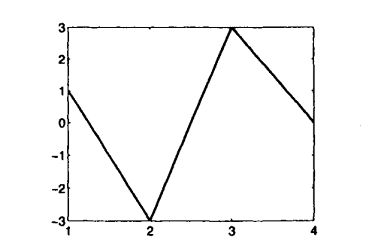
\includegraphics[width=0.8\textwidth,height=70mm]{fig11}
\caption{A simple plot resulting from the command plot (x, y) using the vector
x = [1 2 3 4] for x-coordinates and the vector y = [1 - 3 3 0] for corresponding
y-coordinates. \protect\footnotemark[5] }
\label{fig:fig_1_1}
\end{figure}

\footnotetext[5]{Numerous attributes of a MATLAB plot or other graphic can be modified using the various (very
user-friendly) menu options available on the MATLAB graphics window. These include font sizes,
line styles, colors, and thicknesses, axis label and tick locations, and numerous other items. To
improve readability of this book we will use such features without explicit mention (mostly to make the
fonts more readable to accommodate reduced figure sizes).}

Next, we use the same vector approach to graph the function y = cos($x^2$)
on [0,5]. The finer the grid determined by the vectors you use, the greater the
resolution. To see this first hand, enter: 

\begin{verbatim}
>> x = linspace(0,5,5);               % I will be supressing a lot of output, you
>> 			                                   % can drop the ';' to see it
>> y = cos(x.^2); 
\end{verbatim}

Note the dot (.) before the power operator (\^{}). The dot before an operator
changes the default matrix operation to a \textbf{component-wise operation.} Thus x.\^{}2 
will create a new vector of the same size as $x$ where each of the entries is just the
square of the corresponding entry of $x$. This is what we want. The command x\^{}2
would ask MATLAB to multiply the matrix (or row vector) $x$ by itself, which (as
we will explain later) is not possible and so would produce an error message. 

\begin{verbatim}
>> plot(x,y)  % produces our first very rough plot of the function
>> %  with only 5 plotting points
\end{verbatim}

See Figure 1.2(a) for the resulting plot. Next we do the same plot but using 25
points and then 300 points. The editing techniques of Section 1.2 will be of use
as you enter the following commands. 

\begin{verbatim}
>>x = linspace(0,5,25);
>>y = cos(x. 2);
>>plot(x,y) % a better plot with 25 points.
>>x = linspace(0,5,300);
>>y = cos(2);
>> plot(x,y) % the plot is starting to look good with 300 points. 
\end{verbatim}


\begin{figure}[H]
\centering
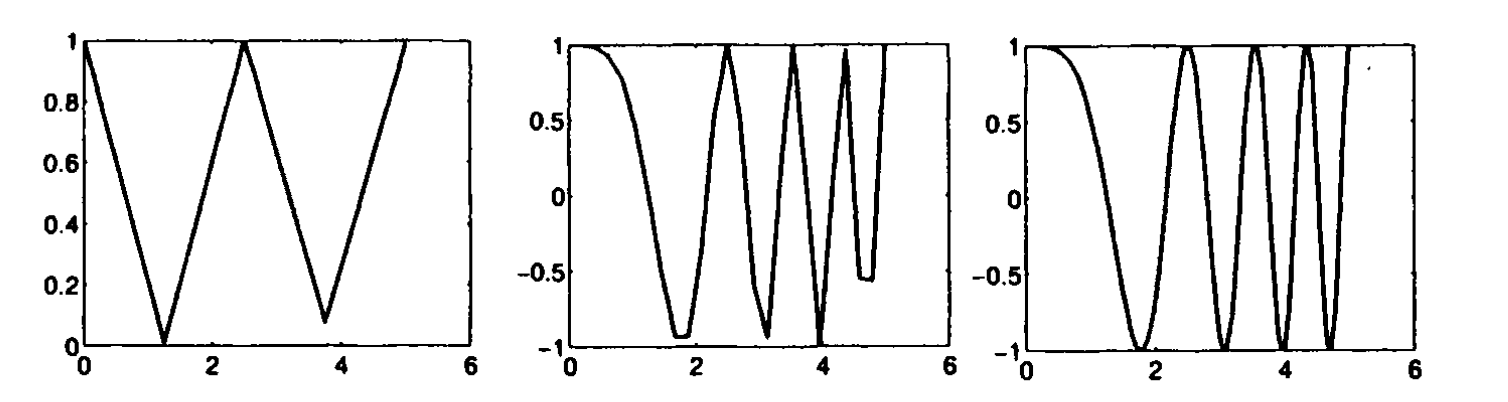
\includegraphics[width=0.8\textwidth,height=30mm]{fig12}
\caption{Plots of the function $y = cos(x^2)$ on [0,5] with increasing resolution: (a)
(left) 5 plotting points, (b) (middle) 25 plotting points, and (c) (right) 300 plotting points. }
\label{fig:fig_1_2}
\end{figure}

If you want to add more graphs to an existing plot, enter the command:

\begin{verbatim}

>> hold on %do this!

\end{verbatim}

All ftiture graphs will be added to the existing one until you enter $hold off$. To
see how this works, let's go ahead and add the graphs of
$y = cos(2x)$ and $y = cos^2x$ to our existing plot of y = cos($x^2$) on [0,5]. To
distinguish these plots, we might want to draw the curves in different styles and
perhaps even different colors. Table 1.1 is a summary of the codes you can use in
a MATLAB plot command to get different plot styles and colors: 

\begin{table}[H]
\caption{ MATLAB codes for plot colors and styles.  }
\centering
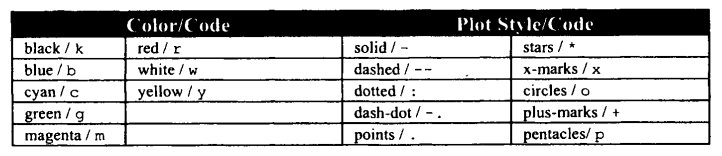
\includegraphics[width=0.8\textwidth,height=30mm]{tab11}
\label{tab:tab_1_1}
\end{table}

Suppose that we want to produce a dashed cyan graph of $y = cos(2x)$ and a
dotted red graph of $y = cos^2x$ (to be put in with the original graph). We would
enter the following:

\begin{verbatim}
>>y1 = cos (2*x);
>>plot(x,y1,'c--') %will plot with cyan dashed curve
>>y2 = cos(x).^2; % cos(x)^2 would produce an error
>>plot(x,y2,'r:') %will plot in dotted red style
>>hold off %puts an end to the current graph
\end{verbatim}

\noindent You should experiment now with a few other options. Note that the last four of
the plot styles will put the given object (stars, x-marks, etc.) around each point that
is actually plotted. Since we have so many points (300) such plots would look like
very thick curves. Thus these last four styles are more appropriate when the
density of plot points is small. You can see the colors on your screen, but unless you have a color printer you should make use of the plot styles to distinguish
between multiple graphs on printed plots.

Many features can be added to a plot. For example, the steps below show how to
label the axes and give your plot a title. 

\begin{verbatim}
>>xlabel('x')
>>ylabel (cos (x.^2), cos(2*x), cos(x).^2') 
>> title('Plot created by yourname') 
\end{verbatim}

Notice at each command how your plot changes; see Figure 1.3 for the final result

\begin{figure}[H]
\centering
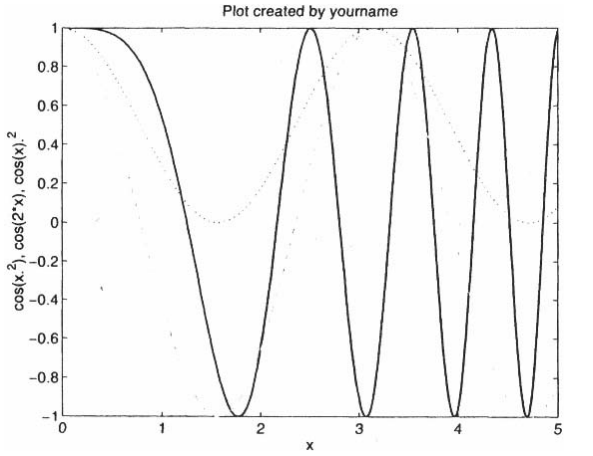
\includegraphics[width=0.8\textwidth,height=100mm]{fig13}
\caption{Plot of three different trigonometric functions done using different colors
and styles }
\label{fig:fig_1_3}
\end{figure}

In a MATLAB plot, the points and connecting line segments need not define the
graph of a function. For example, to get MATLAB to draw the unit square with
vertices (0,0), (1,0), (1,1), (0,1), we could key in the x- and y-coordinates (in an
appropriate order so the connecting segments form a square) of these vertices as
row vectors. We need to repeat the first vertex at the end so the square gets closed
off. Enter

\begin{verbatim}
>>x=[0 1 1 0 0] ; y=[0 0 1 1 0] ;
>>plot(x,y) 
\end{verbatim}

Often in mathematics, the variables x and y are given in terms of an auxiliary
variable, say / (thought of as time), rather than y simply being given in terms of
(i.e., a function of) x . Such equations are called \textbf{parametric equations}, and are easily graphed with MATLAB. Thus parametric equations (in the plane) will look like: 
\[\begin{cases}
    x = x(t)\\
    y = y(t) 
  \end{cases}
\]

These can be used to represent any kind of curve and are thus much more versatile
than functions y = f(x) whose graphs must satisfy the vertical line test.
MATLAB's plotting format makes plotting parametric equations a simple task.
For example, the following parametric equations

\[\begin{cases}
    x = 2cos(t)\\
    y = 2sin(t) 
  \end{cases}
\]
represent a circle of radius 2 and center (0,0). (Check that they satisfy the
equation $x^2  + y^2  = 4$.) To plot the circle, we need only let / run from 0 to 2/$\pi$
(since the whole circle gets traced out exactly once as / runs through these
values). Enter: 

\begin{verbatim}
>>t = 0:.01:2*pi; % a lot of points for decent resolution , as you 
>>			% guessed, 'pi ' is how MATLAB denotes $\pi$
>>x = 2*cos(t);
>>y = 2*sin(t);
>>plot(x,y )
\end{verbatim}


\begin{figure}[H]
\centering
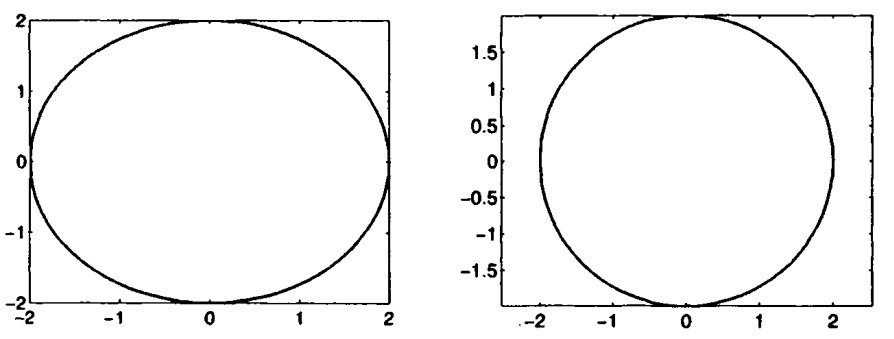
\includegraphics[width=0.8\textwidth,height=45mm]{fig14}
\caption{Parametric plots of the circle x$^2$  + y$^2$  = 4, (a) (left) first using MATLAB's default rectangular axis setting, and then (b) (right) after the command axis (' equal ') to put the axes into proper perspective. }
\label{fig:fig_1_4}
\end{figure}

You will see an ellipse in the figure window (Figure 1.4(a)). This is because MATLAB uses different scales on the x- and y-axes, unless told otherwise. If you enter:>>axis (`equal f' ), MATLAB will use the same scale on both axes so the circle appears as it should (Figure 1.4(b)). Do this!\\

EXERCISE FOR THE READER 1.2: In the same fashion use MATLAB to create
a plot of the more complicated parametric equations:

\[\begin{cases}
    x(t) = 5cos(t/5) + cos(2t) \hspace{0.25cm} for  0<f<10\pi \\
    y(t) = 5sin(t/5) + sin(3t)
  \end{cases}
\]

\textbf{Caution: }  Do not attempt to plot this one by hand!

If you use the axis (' equal ') command in Exercise for the Reader 1.2, you
should be getting the plot pictured in Figure 1.5.

\begin{figure}[H]
\centering
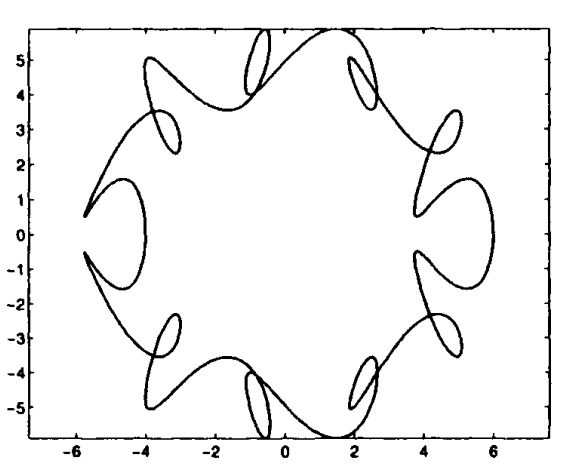
\includegraphics[width=0.8\textwidth,height=75mm]{fig15}
\caption{A complicated MATLAB parametric plot. }
\label{fig:fig_1_5}
\end{figure}

\hrule width \hsize \kern 1pt \hrule width \hsize height 0.4pt

\hspace{0.1cm}

\textbf{EXERCISES 1.4: }

\begin{enumerate}
\item Use MATLAB to plot the graph of $sin(x^4)  for \ {}0 \le x \le  2\pi$, (a) using 200 plotting points, and (b) using 5000 plotting points. 
\item Use MATLAB to plot the graph of $y =e^{(-1/x^2)} for -3 \le x \le  3$, (a) using 50 plotting points, and
(b) using 10,000 plotting points. 

$
\begin{array}{|l|l|}
\hline \begin{array}{l}
\text {axis([xmin xmax ymin ymax] } \rightarrow \\
\end{array} & \begin{array}{l}
\text {Resets the axis range for plots to be: } \\
\text {xmin $\leq$ x $\leq$ xmax }\\
\text {ymin $\leq$ y $\leq$ ymax }\\
\text{Here, the four vector entries can be any real numbers }\\
\text {with xmin < xmax, and ymin < ymax}

\end{array} \\
\hline
\end{array}
$\\

\item Use MATLAB to produce a nice plot of the graph of $y=\frac{2-x^{2}}{x^{2}+x-6}$ on the interval $[-5,5]$. Experiment a bit with the axis command as explained in the above note.
\item Use MATLAB to plot the graph of $y=\frac{x^{4}-16}{x^{3}+2 x^{2}-6}$ on the interval $[-1,5]$. Adjust the axes, as explained in the note preceding Exercise 3, so as to get an attractive plot.
\item Use MATLAB to plot the circle of radius 3 and center $(-2,1)$.
\item Use MATLAB to obtain a plot of the epicycloids that are given by the following parametric 

\begin{equation}
\left\{\begin{array}{l}
x(t)=(R+r) \cos t-r \cos \left(\frac{R+r}{r} t\right) \\
y(t)=(R+r) \sin t-r \sin \left(\frac{R+r}{r} t\right)
\end{array}, 0 \leq t \leq 2 \pi\right.
\end{equation}

equations:
using first the parameters $R=4, r=1$, and then $R=12, r=5$. Use no less than 1000 plotting points.

\textbf{Note:} An epicycloid describes the path that a point on the circumference of a smaller circle (of radius $\mathrm{r}$ ) makes as it rolls around (without slipping) a larger circle (of radius $R$ ).
\item Use MATLAB to plot the parametric equations:
$$
\left\{\begin{array}{l}
x(t)=e^{-\sqrt{t}} \cos (t) \\
y(t)=e^{-\sqrt{2 t}} \sin (t)
\end{array}, 0 \leq t \leq 100 .\right.
$$
\item  Use MATLAB to produce a plot of the linear system (two lines):
$$
\left\{\begin{array}{l}
2 x+3 y=13 \\
2 x-y=1
\end{array}\right.
$$
Include a label for each line as well as a label of the solution (that you can easily find by hand), all produced by MATLAB.

\textbf{Hints:} You will need the hold on command to include so many things in the same graph. To insert the labels, you can use either of the commands below to produce the string of text label at the coordinates $(x, y)$.

$
\begin{array}{|l|l|}
\hline \begin{array}{l}
\text {  text(x, y, ' label ') } \rightarrow \\
\end{array} & \begin{array}{l}
\text { Inserts the text string label in the current graphic window } \\
\text {at the location of the specified point $(x, y)$ }
\end{array} \\
\hline \begin{array}{l}
\text { gtext ('label') } \rightarrow \\
\end{array} & \begin{array}{l}
\text {Inserts the text string label in the current graphic window } \\
\text {at the location of exactly where you click your mouse. }
\end{array} \\
\hline
\end{array}
$\\

\item Use MATLAB to draw a regular octagon (stop-sign shape). This means that all sides have the same length and all interior angles are equal. Scale the axes accordingly.
\item By using the plot command (repeatedly and appropriately), get MATLAB to produce a circle inscribed in a triangle that is in 

\begin{figure}[H]
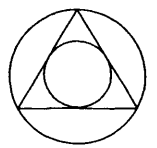
\includegraphics[width=0.20\textwidth,height=20mm,right]{fig16}
\caption{ Illustration for Exercise 10.}
\end{figure}

\item By using the plot command (repeatedly and appropriately), get MATLAB to produce something as close as possible to the familiar figure on the right. Do not worry about the line/curve thickness for now, but try to get it so that the eyes (dots) are reasonably visible.
\begin{figure}[H]

\includegraphics[width=0.20\textwidth,height=20mm,right]{face}
\end{figure}

\end{enumerate}

\section{A TUTORIAL INTRODUCTION TO RECURSION ON MATLAB}

Getting a calculator or computer to perform a single task is interesting, but what
really makes computers such powerful tools is their ability to perform a long series
of related tasks. Such multiple tasks often require a program to tell the computer
1.5: A Tutorial Introduction to Recursion on MATLAB IS
what to do. We will get more into this later, but it is helpful to have a basic idea at
this point of how this works. We will now work on a rather elementary problem
from finance that will actually bring to light many important concepts. There are
several programming commands in MATLAB, but this tutorial will focus on just
one of them (while ) that is actually quite versatile. \\

PROBLEM: To pay off a $\$ 100,000.00$ loan, Beverly pays $\$ 1,000.00$ at the end of each month after having taken out the loan. The loan charges $8 \%$ annual interest (=8/12\% monthly interest) compounded monthly on the unpaid balance. Thus, at the end of the first month, the balance on Beverly's account will be (rounded to two decimals): $\$ 100,000$ (prev. balance) $+\$ 666.27$ (interest rounded to two decimals) $-\$ 1,000$ (payment) $=\$ 99,666.67$. This continues until Beverly pays off the balance; her last payment might be less than $\$ 1,000$ (since it will need to cover only the final remaining balance and the last month's interest).

\begin{enumerate}[label=(\alph*)]
\item Use MATLAB to draw a plot of Beverly's account balances (on the $y$-axis) as a function of the number of months (on the $x$-axis) until the balance is paid off.
\item  Use MATLAB to draw a plot of the accrued interest (on the $y$-axis) that Beverly has paid as a function of the number of months (on the $x$-axis).
\item How many years + months will it take for Beverly to completely pay off her loan? What will her final payment be? How much interest will she have paid off throughout the course of the loan?
\item Use MATLAB to produce a table of values, with one column being Beverly's outstanding balance given in yearly (12 month) increments, and the second column being her total interest paid, also given in yearly increments. Paste the data you get into your word processor to produce a cleaner table of this data.
\item Redo part (c) if Beverly were to increase her monthly payments to $\$ 1,500$.

\end{enumerate}

Our strategy will be as follows: We will get MATLAB to create two vectors B
and TI that will stand for Beverly's account balances (after each month) and the
total interest accrued. We will set it up so that the last entry in B is zero,
corresponding to Beverly's account finally being paid off. \\

There is another way to construct vectors in MATLAB that will suit us well here. We can simply assign the entries of the vector one by one. Let's first try it with the simple example of the vector $x=\left[\begin{array}{lll}1 & 5 & -2\end{array}\right]$. Start a new MATLAB session and enter:


\begin{verbatim}
>>x(1) = 1 %specifies the first entry of the vector x, at this point
>> 		%x will only have one entry 
>>x(2) = 5 %you will see from the output x now has the first two of 
>>		%its three components 
>>x(3) = -2
\end{verbatim}

The trick will be to use \textbf{recursion formulas} to automate such a construction of B
and TI. This is possible since a single formula shows how to get the next entry of
B or TI if we know the present entry. Such formulas are called recursion formulas
and here is what they look like in this case:

$$
\begin{aligned}
&\mathrm{B}(i+1)=\mathrm{B}(i)+(.08 / 12) \mathrm{B}(i)-1000 \\
&\mathrm{TI}(i+1)=\mathrm{TI}(i)+(.08 / 12) \mathrm{B}(i)
\end{aligned}
$$
In words: The next month's account balance $(B(i+1))$ is the current month's balance $(\mathrm{B}(i))$ plus the month's interest on the unpaid balance $((.08 / 12) \mathrm{B}(i))$ less Beverly's monthly payment. Similarly, the total interest accrued for the next month equals that of the current month plus the current month's interest. \\

Since these formulas allow us to use the information from any month to get that for the next month, all we really need are the initial values $B(1)$ and $T I(1)$, which are the initial account balance (after zero months) and total interest accrued after zero months. These are of course $\$ 100,000.00$ and $\$ 0.00$, respectively.\\

\textbf{Caution:} It is tempting to call these initial values $B(0)$ and $T I(0)$, respectively. However this cannot be done since they are, in MATLAB, vectors (remember, as far as numerical data is concerned: Everything in MATLAB is a matrix [or a vector]!) rather than functions of time, and indices of matrices and vectors must be positive integers $(i=1,2, \ldots)$. This takes some getting used to since $i$, the index of a vector, often gets mixed up with $t$, an independent variable, especially by novice MATLAB users.\\

We begin by initializing the two vectors B and T I as well as the index $i$.

\begin{verbatim}

>>B(1)=100000; TI(1)=0; i=1; 

\end{verbatim}

Next, making use of the recursion formulas, we wish to get MATLAB to figure
out all of the other entries of these vectors. This will require a very useful device
called a "while loop". We want the while loop to keep using the recursion
formulas until the account balance reaches zero. Of course, if we did not stop
using the recursion formulas, the balance would keep getting more and more
negative and we would get stuck in what is called an \textbf{infinite loop}. The format for
a while loop is as follows: 

\begin{figure}[H]
\centering
\begin{boxedverbatim}
>>while   <condition>
...MATLAB commands
>>end
\end{boxedverbatim}
\end{figure}


The way it works is that if the <condition> is met, as soon as you enter end, the
"...MATLAB commands..." within the loop are executed, one by one, just as if
you were typing them in on the command window. After this the <condition> is
reevaluated. If it is still met, the "...MATLAB commands..." are again executed
in order. If the <condition> is not met, nothing more is done (this is called exiting
the loop). The process continues. Either it eventually terminates (exits the loop)
or it goes on forever (an infinite loop—a bad program). Let's do a simple example before returning to our problem. Before you enter the following
commands, try to guess, based on how we just explained while loops, exactly what
MATLAB's output will be. Then check your answer with MATLAB's actual
output on your screen. If you get it right you are starting to understand the concept
of while loops. 

\begin{verbatim}
>>a=1;
>>while a^2 < 5 * a
	 a=a+2, a^2
     end 
\end{verbatim}

EXERCISE FOR THE READER 1.3: Analyze and explain each iteration of the
above while loop. Note the equation $a=a+2$ in mathematics makes no sense at
all. But remember, in MATLAB the single equal sign means "assignment." So
for example, initially $a = 1$. The first run through the while loop the condition is
met ($1 = a^2 < 5a = 5$ ) so a gets reassigned to be 1 + 2 = 3, and in the same line $a^2$
is also called to be computed (and listed as output).\\

Now back to the solution of the problem. We want tto continue using the above
recursion formulas as long as the balance  $B(i)$ remains positive. Since we have
already initialized $B(1)$ and $TI(1)$, one possible MATLAB code for creating the
rest of these vectors would look like: 

\begin{verbatim}
>>while B(i) > 0
	B(i+1)=B(i)+ 8/12/100*B(i)-1000; % This and the next are just our recursion formulas. 
	TI(i+1)=TI(i)+ 8/12/100*B(i);
	  i=i+1; % this bumps the vector index up by one at each  iteration.
end
\end{verbatim}

Notice that MATLAB does nothing, and the prompt does not reappear again, until
the while loop is closed off with an end (and you press enter). Although we have
suppressed all output, MATLAB has done quite a lot; it has created the vectors B
and $TI$. Observe also that the final balance of zero should be added on as a final
component. There is one subtle point that you should be aware of: The value of
i after the termination of the while loop is precisely one more than the number of
entries of the vectors $B$ and $TI$ thus far created. Try to convince yourself why this
is true! Thus we can add on the final entry of B to be zero as follows: 

\begin{verbatim}
>> n=i; B(n)=0; %We could have just typed 'B(i)=0' but we wanted to 
			>>% call 'n' the length of the vector B.
\end{verbatim}

Another subtle point is that $B(n)$ was already assigned by the while loop (in the
final iteration) but was not a positive balance. This is what caused the while loop
to end. So what actually will happen at this stage is that Beverly's last monthly
payment will be reduced to cover exactly the outstanding balance plus the last
month's interest. Also in the final iteration, the total interest was correctly given
by the while loop. To do the required plots, we must first create the time vector.
Since time is in months, this is almost just the vector formed by the indices of B
(and TI), i.e., it is almost the vector [1 2 3 ... n]. But remember there is one
slight subtle twist. Time starts off at zero, but the vector index must start off at 1.
Thus the time vector will be [0 1 2 ... n - 1]. We can easily construct it in
MATLAB by 

\begin{verbatim}
>>t=0:n-1; %this is shorthand for `'t=0:1:n-1', by default the
>>		% gap size is one.
\end{verbatim}

Since we now have constructed all of the vectors, plotting the needed graphs is a
simple matter. 

\begin{verbatim}
>>plot(t,B)
>>xlabel('time in months'), ylabel ('unpaid balance in dollars')
>> 		%we add on some descriptive labels on the horizontal and vertical
>> 		%axis. Before we go on we copy this figure or save it (it is
>> 		%displayed below)
>>plot(t, TI) 
>> xlabel('time in months'), ylabel('total interest paid in dollars')
\end{verbatim}

See Figure 1.7 for the MATLAB graphics outputs.

\begin{figure}[H]
\centering
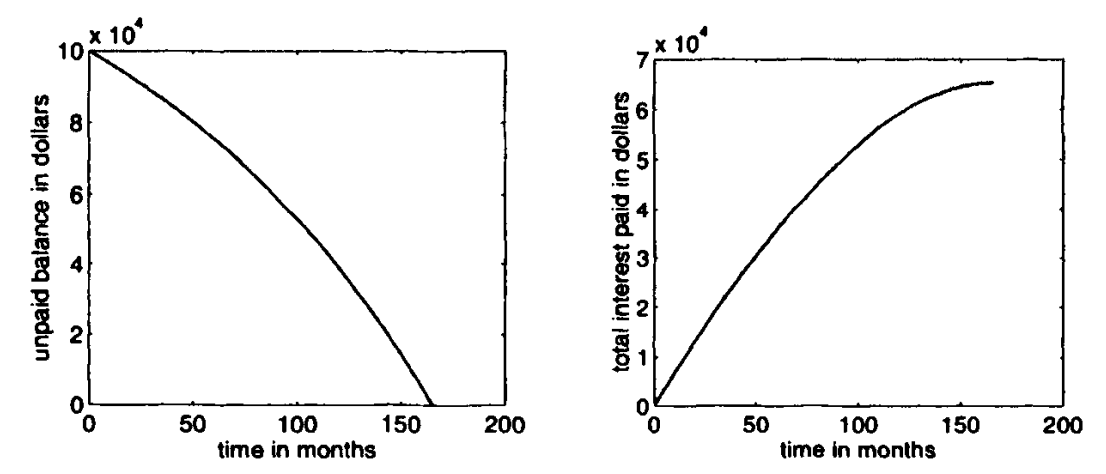
\includegraphics[width=0.8\textwidth,height=55mm]{fig17}
\caption{(a) (top) Graph of the unpaid balance in dollars, as a function of elapsed
months in the loan of \$100,000 that is being analyzed, (b) (bottom) Graph of the total
interest paid in dollars, as a function of elapsed months in the loan of \$100,000 that is being
analyzed. }
\label{fig:fig_1_7}
\end{figure}

We have now taken care of parts (a) and (b). The answer to part (c) is now well
within reach. We just have to report the correct components of the appropriate
vectors. The time it takes Beverly to pay off her loan is given by the last value of
the time vector, i.e.,

\begin{verbatim}
>>n-1
->166.00 =13 years + 10 months (time of loan period).
\end{verbatim}

Her final payment is just the second-to-last component of B, with the final month's
interest added to it (that's what Beverly will need to pay to totally clear her
account balance to zero):

\begin{verbatim}
>>format bank % this puts our dollar answers to the nearest cent.
>>B(n-1)*(1+8/12/100) 
>>$341.29 (last payment).
\end{verbatim}

The total interest paid is just: 

\begin{verbatim}
>>TI(n) 
->$65,341.29 (total interest paid)
\end{verbatim}

Part (d): Here we simply need to display parts of the two vectors, corresponding
to the ends of the first 13 years of the loan and finally the last month (the 10th
month after the 13th year). To get MATLAB to generate these two vectors, we
could use a while loop as follows:\footnote[6]{A slicker way to enter these vectors would be to use MATLAB's special vector-creating construct
that we mentioned earlier as follows: YB = B (1:12:167), and similarly for YTI. }

\begin{verbatim}
>> k=1; i=1; \%we will use two indices, k will be for the original
>>\% vectors, i will be for the new ones.
>>while k<167
		 YB(i)=B(k); YTI(i)=TI(k); %we create the two new "yearly" vectors. 
		 k=k+12; i=i+1; %at each iteration, the index of the original
					%vectors gets bumped up by 12, but that for
					%the new vectors gets bumped up only by one.
end 
\end{verbatim}


We next have to add the final component onto each vector (it does not correspond
to a year's end). To do this we need to know how many components the yearly
vectors already have. If you think about it you will see it is 14, but you could have
just as easily asked MATLAB to tell you: 

\begin{verbatim}
>> size(YB) %this command gives the size of any matrix or vector
			% (\# of rows, \# of columns).
->ans = 1.00 14.00
>>YB(15)=B(167); YTI(15)=TI(167);
>>YB=YB'; YTI=YTI'; % this command reassigns both yearly vectors to
				% be column vectors
\end{verbatim}

Before we print them, we would like to print along the left side the column vector
of the corresponding years' end. This vector in column form can be created as
follows: 

\begin{verbatim}
>>years = 0:14; years = years' %first we create it as a row vector
>>					%and then transpose it.
\end{verbatim}

We now print out the three columns: 

\begin{verbatim}
>>years, YB, YTI % or better (years, YB, YTI)
\end{verbatim}

\noindent \begin{tabular}{ccc}
years=  &YB=  &YTI=  \\
		0&100000.00&0\\

		1.00&95850.02&7850.02\\

		2.00&91355.60&15355.60\\

		3.00&86488.15&22488.15\\

		4.00&81216.69&29216.69\\

		5.00&75507.71 &35507.71\\

		6.00&69324.89&41324.89\\
		
		7.00&62628.90&46628.90\\
		
		8.00&55377.14&51377.14\\
		
		9.00&47523.49&55523.49\\
		
		10.00&39017.99&59017.99\\
		
		11.00&29806.54&61806.54\\
		
		12.00&19830.54&63830.54\\
		
		13.00&9026.54 &65026.54\\
		
		14.00&0.00&65341.29\\
\end{tabular}

Finally, by making use of any decent word processing software, we can embellish
this rather raw data display into a more elegant form such as Table 1.2. 

\begin{table}[H]
\caption{Summary of annual data for the \$100,000 loan that was analyzed in this
section. 
  }
\centering
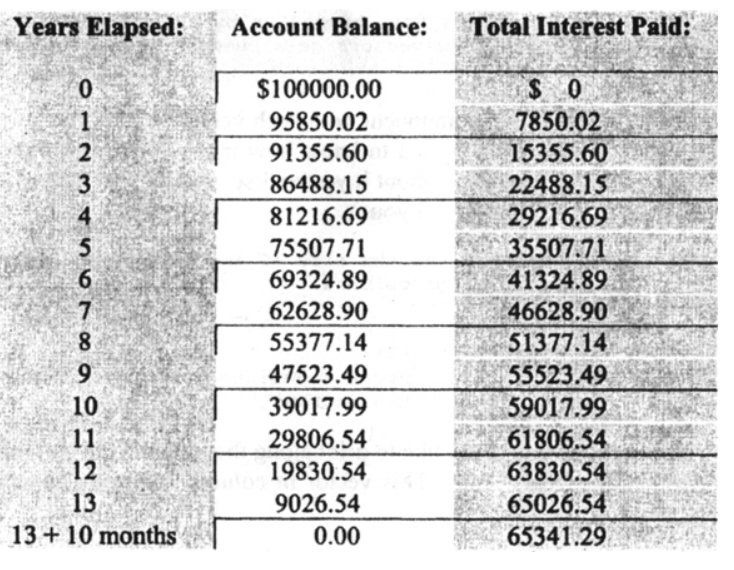
\includegraphics[width=0.8\textwidth,height=100mm]{tab14}
\label{tab:tab_1_4}
\end{table}

Part (e): We can run the same program but we need only modify the line with the 
recursion formula for the vector B: It now becomes:$ B(i + 1) = B(i)+I( i + 1)-1500;$ . With this done, we arrive at the following data: 

\begin{verbatim}
>>i-1, B(i-1)*(1+8/12/100) , TI(i)
->89 (7 years + 5 months),\$693.59(last pmt), \$32693.59 (total interest paid)

\end{verbatim}

\hrule width \hsize \kern 1pt \hrule width \hsize height 0.4pt

\hspace{0.1cm}

\textbf{EXERCISES 1.5: }


\begin{enumerate}

\item Use a while loop to add all of the odd numbers up: 1 + 3 + 5 + 7 + · · · until the sum exceeds 5 
million. What is the actual sum? How many odd numbers were added?

\item Redo Exercise 1 by adding up the even numbers rather than the odd ones.

\item\emph{(Insects from Hell)} An insect population starts off with one pair at year zero. The insects are 
immortal (i.e., they never die!) and after having lived for two years each pair reproduces another 
pair (assumed male and female). This continues on indefinitely. So at the end of one year the 
insect population is still 1 pair (= 2 insects); after two years it is 1 + 1 = 2 pairs (= 4 insects), 
since the original pair of insects has reproduced. At the end of the third year it is 1 + 2 = 3 
pairs (the new generation has been alive for only one year, so has not yet reproduced), and after 
4 years the population becomes 2 + 3 = 5 pairs, (a) Find out the insect population (in pairs) at 
the end of each year from year 1 through year 10. (b) What will the insect population be at the 
end of 64 years? 

HISTORICAL ASIDE: The sequence of populations in this problem: 1,1,1 + 1=2 , 1+ 2 = 3, 2 + 3 
= 5,3 + 5 = 8,... was first introduced in the middle ages by the Italian mathematician Leonardo of Pisa 
(ca. 1180-1250), who is better known by his nickname: Fibonacci (Italian, meaning son ofBonaccio). 
This sequence has numerous applications and has made Fibonacci quite famous. It comes up, for 
example, in hereditary effects in incest, growth of pineapple cells, and electrical engineering. There is 
even a mathematical journal named in Fibonacci's honor (the Fibonacci Quarterly). 

\item Continuing Exercise 3, (a) produce a chart of the insect populations at the end of each 10th year 
until the end of year 100. (b) Use a while loop to find out how many years it takes for the insect 
population (in pairs) to exceed 1,000,000,000 pairs. 

\item \emph{(Another Insect Population Problem)} In this problem, we also start off with a pair of insects, 
this time mosquitoes. We still assume that after having lived for two years, each pair reproduces 
another pair. But now, at the end of three years of life, each pair of mosquitoes reproduces one 
more pair and then immediately dies, (a) Find out the insect population (in pairs) for each year 
up through year 10. (b) What will the insect population be at the end of 64 years?

\item Continuing Exercise 5, (a) plot the mosquito (pair) population from the beginning through the 
end of year 500, as a function of time, (b) How many years does it take for the mosquito 
population (in pairs) to exceed 1,000,000,000 pairs? 

\item When their daughter was born, Mr. and Mrs. de la Hoya began saving for her college education 
by investing \$5,000 in an annuity account paying 10\% interest per year. Each year on their 
daughter's birthday they invest \$2,000 more in the account, (a) Let A„ denote the amount in 
the account on their daughter's wth birthday. Show that An satisfies the following recursion 
formulas: 

\begin{equation}
\begin{aligned}
&A_{0}=5000 \\
&A_{n}=(1.1) A_{n-1}+2000 .
\end{aligned}
\end{equation}

(b) Find the amount that will be in the account when the daughter turns 18. 

(c) Print (and nicely label) a table containing the values of n and An as n runs from 0 to 18.

\item Louise starts an annuity plan at her work, that pays 9% annual interest compounded monthly. 
She deposits \$200 each month starting on her 25th birthday. Thus at the end of the first month 
her account balance is exactly\$200. At the end of the second month, she puts in another \$200, 
but her first deposit has earned her one month's worth of interest. The 9% interest per year 
means she gets 9\%/12 = 0.75\% interest per month. Thus the interest she earns in going from the 
first to second month is .75\% of \$200 or\$ 1.50, and so her balance at the end of the second 
month is 401.50. This continues, so at the end of the 3rd month, her balance is \$401.50 (old balance) + .75\% of this (interest) + \$200 (new deposit) = \$604.51. Louise continues to do this 
throughout her working career until she retires at age 65. 

(a) Figure out the balances in Louise's account at her birthdays: 26th, 27th, ..., up through her 
65th birthday. Tabulate them neatly in a table (either cut and paste by hand or use your word 
processor—do not just give the raw MATLAB output, but rather put it in a form so that your 
average citizen could make sense of it). 

(b) At exactly what age (to the nearest month) is Louise when the balance exceeds \$100,000? 
Note that throughout these 40 years Louise will have deposited a total of \$200/month x 12 
months/yr. x 40 years = \$96,000. 

\item In saving for retirement, Joe, a government worker, starts an annuity that pays 12% annual 
interest compounded monthly. He deposits \$200.00 into it at the end of each month. He starts 
this when he is 25 years old. (a) How long will it take for Joe's annuity to reach a value of \$1 
million? (b) Plot Joe's account balance as a function of time. 
 
\item The dot product of two vectors of the same length is defined as follows:

If
$$
x=[x(1) x(2) \cdots x(n)], y=[y(1) y(2) \cdots y(n)]
$$
then
$$
x \cdot y=\sum_{i=1}^{n} x(i) y(i)
$$

The dot product appears and is useful in many areas of math and physics. As an example, check that the dot product of the vectors[2 0 6] and [1 -1  4] is 26 . In MATLAB, if $x$ and $y$ are stored as row vectors, then you can get the dot product by typing $x^{\star} y^{\prime}$ (the prime stands for transpose, as in the previous section; Chapter 7 will explain matrix operations in greater detail). Let $x$ and $y$ be the vectors each with 100 components having the forms:
$$
\begin{aligned}
&x=[1,-1,1,-1,1,-1, \cdots], \\
&y=[1,4,9,16,25,36, \cdots] .
\end{aligned}
$$
Use a while loop in MATLAB to create and store these vectors and then compute their dot product.
 
\end{enumerate}

\clearpage

\end{document} 
